\documentclass[utf8, professionalfonts]{beamer}
\usetheme{Warsaw}

\usepackage[utf8]{inputenc}
\usepackage[english,russian]{babel}

\usepackage{url}
\usepackage{graphicx}
\usepackage{wrapfig}
\graphicspath{{./img/}{../img/}}

%% old \title[Построение структурного выравнивания]{Построение и анализ структурного выравнивания молекул биополимеров в рамках проекта UGENE}
\title[Построение структурного выравнивания]{Инструменты построения и анализа структурного выравнивания молекул биополимеров для проекта UniPro UGENE}
\author[Кузнецов Алексей]{Кузнецов Алексей ФФ гр. 7312 \linebreak научный руководитель Фурсов М.Ю. UniPro}
\institute{Новосибирский Государственный Университет}
\date{\today}

\begin{document}
% Итак, приступим...

\begin{frame}
\titlepage
\end{frame}

% Структурное выравнивание, что это такое
% Это попытка определить гомологичность двух белков
% на основе их третичной структуры
% Термин выравнивание взят по аналогии с выравниванием последовательностей
\begin{frame}{Структурное выравнивание}
\begin{columns}[c]
\column{0.45\linewidth}
	\center{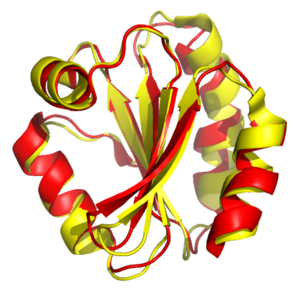
\includegraphics[width=\linewidth]{wiki.png}}
\column{0.55\linewidth}
	Определение гомологичности молекул биополимеров таких как
	\begin{itemize}
		\item Белки
		\item РНК
	\end{itemize}
	по их третичной структуре

\end{columns}

\end{frame}

% Это важный инструмент структурной биологии
% Определение функционального назначения на основе структуры
% Сравнение белков с сильноразличающейся первичной структурой(аминокислотной последовательностью)
% Оценка алгоритмов предсказания структуры
\begin{frame}{Структурное выравнивание}
Важный инструмент структурной биологии, необходимый для

\begin{itemize}
	\item Сравнения и классификации структур
	\item в т.ч. белков с различной аминокислотной последовательностью
	\item Предсказания третичной структуры
	\item Определения функционального назначения молекул
	\item Конструирования искусственных молекул
\end{itemize}

\end{frame}

% Суть метода: выравниваем 2(попарное) или несколько(множественное) молекул
% минимизируя rmsd
\begin{frame}{Суть метода}
\begin{figure}[h]
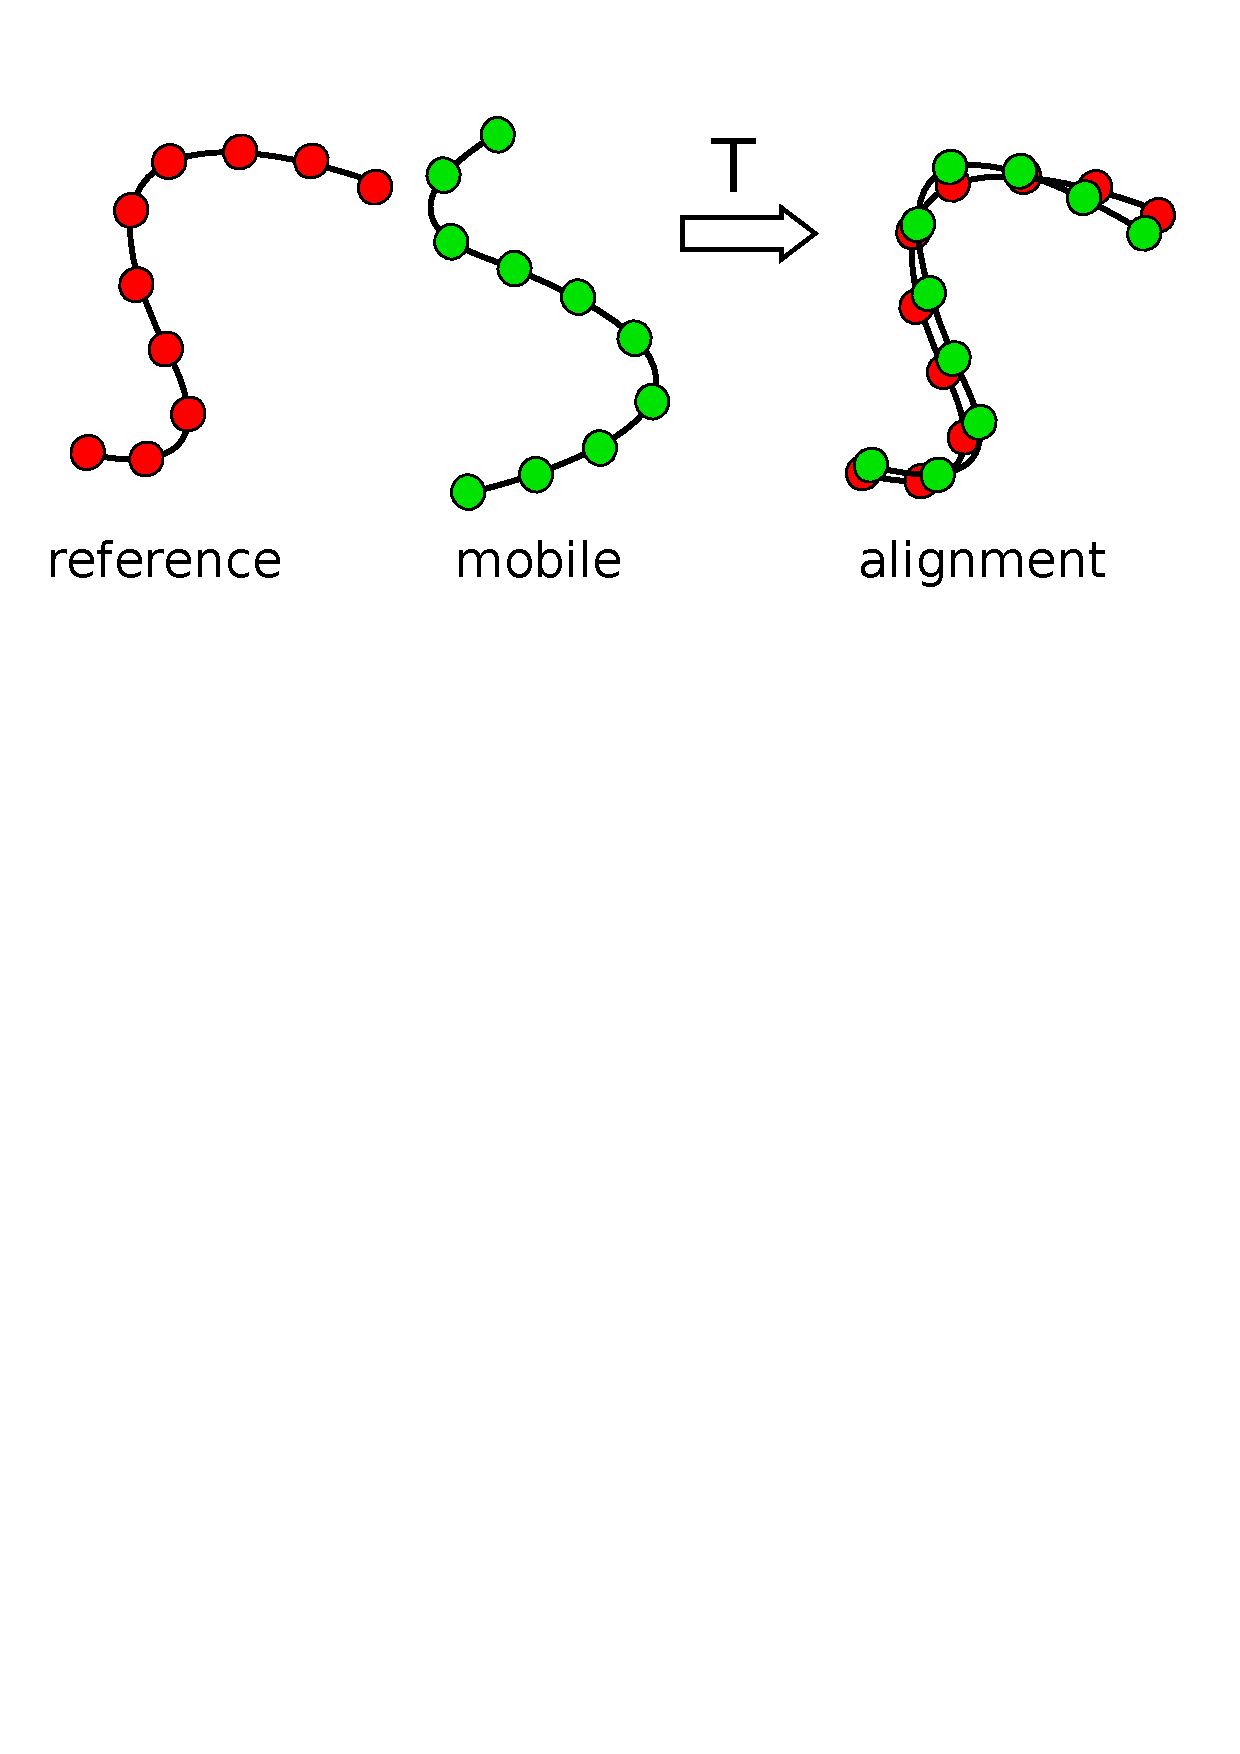
\includegraphics[clip, trim=0 19.5cm 0 1cm, width=\linewidth]{method.pdf}
\end{figure}

Поиск трансформации ({\bf T}) для наилучшего выравнивания, минимизирующего {\bf RMSD} (root mean square deviation)
\begin{math}
\operatorname{RMSD}(ref, mob) = \sqrt{\frac{\sum_{i=1}^n (x_{1,i} - x_{2,i})^2}{n}}
\end{math}

\end{frame}

% Входные данные это третичная структура, попросту 3х-мерная модель
% может усугубляться всякими дополнительными данными
% Источники экспериментальные NMR, X-Ray; смоделированные
% обычно записывается в файлы формата PDB
% Результат rmsd и матрица пребразования
\begin{frame}{Входные данные и результаты}
Входные данные -- трехмерная модель

\begin{itemize}
	\item Измеренная - NMR, X-Ray
	\item Смоделированная - алгоритмы предсказания
\end{itemize}	
Формат -- файлы PDB (\url{http://www.pdb.org})

\vspace{11pt}

Результаты
\begin{itemize}
	\item RMSD - root mean square deviation
	\item Матрица преобразований модели - сдвиг, поворот
\end{itemize}	
Так же можно экспортировать в PDB
\end{frame}

% Слайд с кучей алгоритмов, немногие из них существуют в виде законченных продуктов
\begin{frame}{Существующие алгоритмы}
\begin{center}
\begin{small}
MAMMOTH CE/CE-MC DaliLite VAST PrISM SSAP SARF2 KENOBI/K2 STAMP MASS SCALI DEJAVU SSM SHEBA LGA POSA PyMOL FATCAT Matras MAMMOTH-mult Protein3Dfit PRIDE FAST C-BOP ProFit TOPOFIT MUSTANG URMS LOCK LOCK 2 CBA TetraDA STRAP LOVOALIGN GANGSTA GANGSTA+ TM-align MatAlign Vorolign EXPRESSO CAALIGN YAKUSA BLOMAPS CLEPAPS TALI F MolCom MALECON FlexProt MultiProt CTSS CURVE Matt TopMatch SSGS Matchprot UCSF Chimera  FLASH RAPIDO ComSubstruct ProCKSI SARST Fr-TM-align TOPS+ COMPARISON TOPS++ FATCAT MolLoc FASE SABERTOOTH STON SALIGN MAX-PAIRS THESEUS TABLEAUSearch QP Tableau Search ProSMoS MISTRAL MSVNS for MaxCMO Structal ProBiS ALADYN SWAPSC SA Tableau Search
\end{small}
\end{center}
\end{frame} 

% Пара слов о UGENE. Объединяет множество инструментов в одном формате.
% Уже имеет инструменты выравнивания последовательностей, визуализации макромолекул, ограниченную поддержку PDB
\begin{frame}{UGENE}
\begin{center}
\Large{UniPro UGENE -- это открытое ПО для работы молекулярного биолога}
\end{center}

% Слайд UGENE #1 - Цели проекта, скриншот
\begin{columns}
\column{0.5\linewidth}
	\center{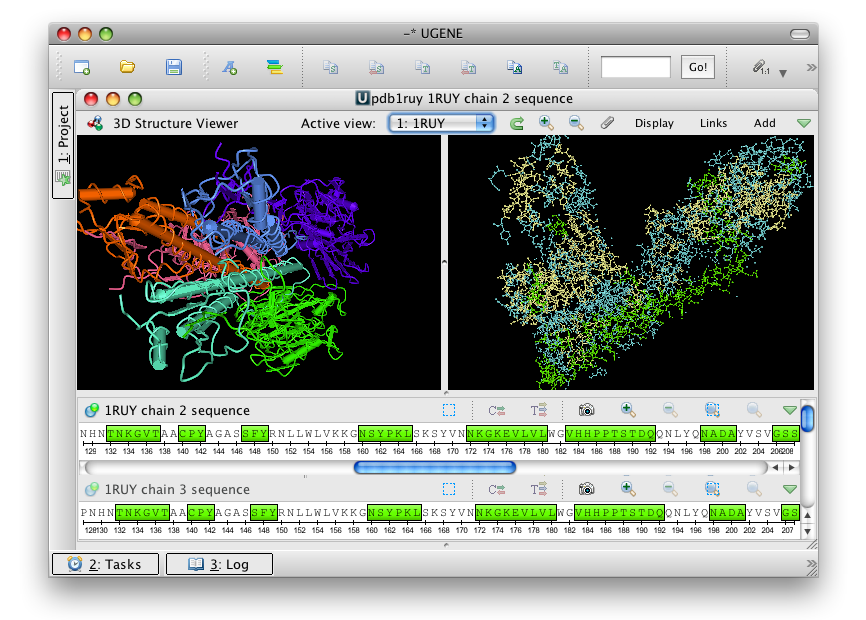
\includegraphics[width=\linewidth]{screen.png}}
	
\column{0.5\linewidth}
	Цель проекта: Качественная интеграция существующих инструментов для биолога в единый графический и вычислительный интерфейс
	
\end{columns}
\end{frame}

% Слайд UGENE #2 - Преимущества, что уже есть
\begin{frame}{Преимущества UGENE}

\begin{columns}[c]
	\column{0.67\linewidth}
		\begin{itemize}
			\item Проект активно развивается
			\item Объединяет десятки популярных инструментов биолога
			\item Более {\bf 10\textsuperscript{6}} строк кода, более {\bf 5000} автоматических тестов
			\item Платформы {\bf Windows}, {\bf Linux} и {\bf Mac}
			\item Входит в официальную поставку дистрибутивов {\bf Ubuntu} и {\bf Fedora}
			\item Сообщество {\bf $\sim$1000} пользователей
			\item Код доступен по лиценззи {\bf GPL} 
			\item публичный багтрекер, форум, видео-подкаст
		\end{itemize}
	
	\column{0.4\linewidth}
		\center{
\includegraphics[width=0.8\linewidth]{gnu.png}}
		\center{
\includegraphics[width=0.8\linewidth]{platforms.png}}
\end{columns}

\end{frame}

% Цель: реализовать такой инструмент в продукте UniPro UGENE
% Задачи: построение, визуализация, импорт/экспорт, оформление, основа для дальнейшего развития
\begin{frame}{Цель работы}
\begin{center}
\Large Реализовать инструменты построения и анализа структурного выравнивания для проекта UGENE
\end{center}
\vspace{11pt}
Задачи
\begin{itemize}
	\item Поиск и интеграция существующего алгоритма 
	\item Интерактивная визуализация выравнивания
	\item Поддержка сохранения/загрузки результатов 
	\item Общий API для алгоритмов выравнивания
	\item Тестирование и покрытие автоматическими тестами
\end{itemize}
\end{frame}

% Результаты
\begin{frame}{Результаты}
\begin{itemize}
	\item Сделан обзор библиотек, выбрана и встроена библиотека {\bf PTools}: an opensource molecular docking library
		\begin{itemize}
			\item[-] Алгоритм Sippl MJ, Stegbuchner H 
			\item[-] Совместимая лицензия GPL
			\item[-] Написана на C/C++
		\end{itemize}
	\item Реализована визуализация выравнивания в BioStruct3D
	\item Добавлена инфраструктура для алгоритмов выравнивания (интерфейсы и типы данных)
	\item Добавлены автоматические тесты
	\item Множество исправлений и улучшений в BioStruct3D

\end{itemize}
\end{frame}


% Спасибо за внимание
\begin{frame}{Q\&A}
\begin{center} 
\LARGE{Спасибо за внимание!}
\end{center}
\end{frame}

\end{document}
